\chapter[Preliminares ]{Preliminares }\label{ch:capitulo3}
En este capítulo presentaremos diversos términos fundamentales. El objetivo principal es entregar un marco teórico sobre los conceptos que se utilizan en los siguientes capítulos para definir las técnicas utilizadas.
\begin{definition}[Celdas]
\label{def:cel}
Una celda consiste en una porción que mide 8x8 pixeles.
\end{definition}
\begin{definition}[Bloques]
\label{def:blo}
Un bloque es una porción de la imagen que corresponde a 2x2 celdas.
\end{definition}

\section{Histogram of Oriented Gradients}
\label{subsec:hog}
\textit{Histogram of Oriented Gradients (HOG)} presentado por Dalal y Triggs~\cite{hog2005}, es un descriptor de características utilizado en visión por computador y procesamiento de imágenes, el cual se utiliza para describir objetos (latas, botellas, autos, personas, rostros, etc). En términos generales, HOG, es una técnica que cuenta las ocurrencias de las orientaciones de los gradiente en partes especificas de una imagen. Este método calcula un espacio de celdas superpuestas con el fin de normalizar las muestras locales y aumentar la precisión.

HOG cuenta con ciertos pasos que se deben realizar para obtener los descriptores de las imágenes, esto se puede ver en la Figura~\ref{fig:hog_procedure}. A continuación se detallan las etapas que componen el algoritmo HOG.
\begin{figure}[tb]
  \centering
   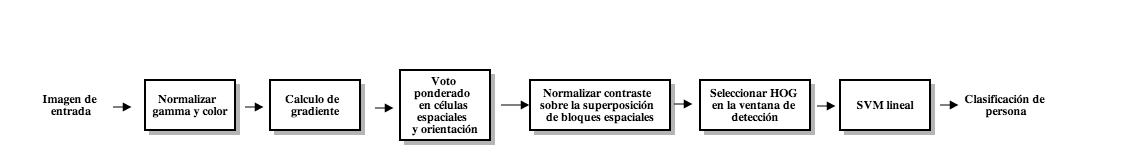
\includegraphics[width=1\textwidth]{Figuras/hog-procedure.png}
   \caption{Procedimiento de HOG}
   \label{fig:hog_procedure}
\end{figure}

\subsection{Procedimiento de HOG}

Como primer paso se define los bloques (ver Definición~\ref{def:blo}), los cuales dividen a la imagen en 16x16 bloques con superposición. Por ejemplo, si una imagen mide 128x128 pixeles, en ella se obtendrían, 15x15 bloques, dando un total de 225 bloques, ver Figura~\ref{fig:blocks_cells}.
\begin{figure}[tb]
  \centering
   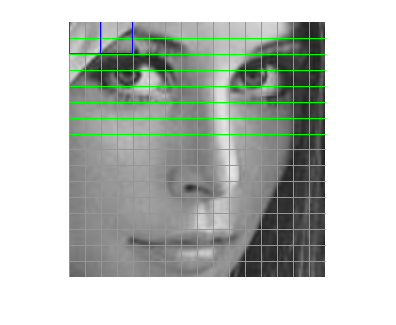
\includegraphics[width=1\textwidth]{Figuras/lena-grid.png}
   \caption{Bloques (azul y rojo), celdas (verde)}
   \label{fig:blocks_cells}
\end{figure}
Se divide la imagen en 16x16 bloques con un 50\% de superposición. Cada uno de estos bloques debiese consistir en celdas de 2x2, donde cada una de ellas tiene una dimensión de 8x8 pixeles. Luego de definir los bloques se cuantiza en nueve espacios (bins) la orientación de los gradientes de 0 a 180 grados. 
\subsubsection{Votación}

\subsubsection{Normalización de superposiciones}

\subsubsection{Selección}

\subsubsection{Linear SVM}

\subsubsection{Detección}

\section{Filtros}
\label{subsec:fl}

\section{Score}
\label{subsec:score}

\section{SVM}
\section{Resumen}

